Wie in \autoref{theorie:referenzmodellierung} beschrieben, müssen Referenzmodelle einen subjektiven Empfehlungscharakter besitzen, damit sie akzeptiert und wiederverwendet werden. Dafür muss ein Abgleich mit den Anforderungen der Nutzenden geschehen. Um dies zu erreichen, wurden im Anhang transkribierte Interviews (vgl. \anhangref{anhang:interview-philipp-22.03.2021}, \anhangref{anhang:interview-peter-24.03.2021}, \anhangref{anhang:interview-ralph-24.03.2021}) durchgeführt. Daraus ergibt sich das in \autoref{abb:TopLevelEchtzeitRA} gezeigte Diagramm, welches die Anforderungen der individuellen Stakeholder an Dekompositionstiefe, Anwendbarkeit und Allgemeingültigkeit darstellt.

\begin{figure}[H]
\centering
\spideroverview
%{Philipp A.}
{5}{3}{3}
%{Ralph B.}
{3}{3}{1}
%{Peter E.}
{2}{4}{5}
\caption{Ergebnisse der Interviews}
\label{abb:DimensionenUebersicht}
\end{figure}
Durch die Interviews ließen sich folgende Durchschnitte errechnen: Dekompositionstiefe wurde im Schnitt mit $3,\overline{3}$ bewertet. Die Anwendbarkeit wurde ebenfalls mit $3,\overline{3}$ bewertet. Die Allgemeingültigkeit hingegen hat nur einen Schnitt von $3$. Entsprechend sollten Dekompositionstiefe und Anwendbarkeit priorisiert werden, während die Referenzarchitektur organisationsspezifischer sein darf. 

Zusätzlich haben sich im Rahmen der Interviews folgende Anforderungen ergeben:
\begin{enumerate}
\item Anwendbarkeit auf Monitoringdaten (IT) (\anhangref{anhang:interview-philipp-22.03.2021}, \anhangref{anhang:interview-peter-24.03.2021})
\item Anwendbarkeit auf Sensordaten (\ac{IoT}) (\anhangref{anhang:interview-philipp-22.03.2021}, \anhangref{anhang:interview-peter-24.03.2021}, \anhangref{anhang:interview-ralph-24.03.2021})
\item Handling von Events, Messwerten und \enquote{Streaming} (\anhangref{anhang:interview-peter-24.03.2021})
\item Automatisierte operative Entscheidungen
\item \label{anforderung:wertschöpfung} Wertschöpfung für das Unternehmen wichtig
\item \label{anforderung:akzeptabel} akzeptabel und problemlösend für Domäne
\item \label{anforderung:zugänglichkeit} Zugänglichkeit und zugang durch Mehrheit der Organisation
\end{enumerate}

Im Folgenden werden die Referenzarchitekturen entworfen und miteinander verglichen, um mögliche Stärken und Einsatzgebiete zu identifizieren. Einige der Anforderungen, wie \ref{anforderung:wertschöpfung}, \ref{anforderung:akzeptabel} und \ref{anforderung:zugänglichkeit} werden nicht für beide Referenzarchitekturen einzeln, sondern gesammelt erfasst.

In den folgenden Referenzarchitekturen wird in mehrere Dekompositionen unterteilt. In der Datenverarbeitungssequenz werden mit Hilfe eines Sequenzdiagramms die Abläufe zur Datenverarbeitung mit dem zu betrachtenden Dienst, ausgehend von \AWSIOT{} Core als Messagebroker, gezeigt.
Die Verteilungssicht soll sowohl die Interaktion der Dienste untereinander, als auch grob das durchzuführende Deployment zeigen. Die Bausteinsicht zeigt wichtige Elemente der einzelnen Dienste auf, die konkret untereinander interagieren. So ist die konkrete Untereinheit, die Daten von \AWSIOT{} Core an andere Dienste versendet, eine \AWSIOT{} Core Rule, welche aufzuzeigen wäre.

Zusätzlich zu den Dekompositionssichten wird auch ein Monitoringkonzept vorgestellt, um Fehler in den Abläufen schnell erkennen zu können. Dieses Monitoringkonzept soll kritische Metriken aufzeigen, welche überwacht werden müssen, um kontinuierliche Analysen sicherzustellen. Für das Monitoringkonzept wird vorausgesetzt, dass der \ac{AWS}-native Dienst CloudWatch zur Überwachung eingesetzt wird. 
\begin{figure}[H]
\centering
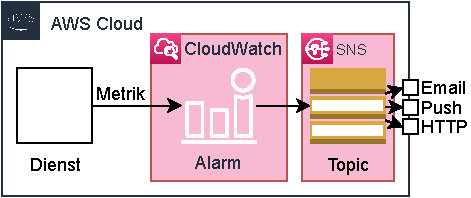
\includegraphics[width=0.66\textwidth]{graphics/CloudWatch-Monitoring}
\caption{CloudWatch Monitoring}
\label{abb:CloudWatchMonitoring}
\end{figure}
CloudWatch erfasst zentralisiert Metriken aller Dienste und löst bei nutzerdefinierten Überschreitungen einen Alarm aus, welcher dann via \ac{SNS} versendet werden kann (siehe \autoref{abb:CloudWatchMonitoring}). Dabei kann bei Metriken mit hoher Varianz die Cloudwatch eigene Anomalienerkennung verwendet werden oder die Schwellwerterkennung.



